\documentclass[12pt]{article}
\usepackage[utf8]{inputenc}

\usepackage{enumitem}
\usepackage[margin=2cm]{geometry}

\usepackage{amsmath, amsfonts, amssymb}
\usepackage{graphicx}
\usepackage{tikz}
\usepackage{pgfplots}
\usepackage{multicol}

\usepackage{comment}
\usepackage[colorlinks=true, urlcolor=blue]{hyperref}
\usepackage{calc}
\usepackage{subcaption}
\usepackage{circledsteps}
\usepackage{wrapfig}
\usepackage{array}
\usepackage{systeme}
\sysdelim..

\setlength\parindent{0pt}

\usepackage{fancyhdr}
\pagestyle{fancy}
\fancyhf{}
\renewcommand{\headrulewidth}{2pt}
\renewcommand{\footrulewidth}{0pt}
\rfoot{\thepage}
\lhead{\textsc{Math} 311}
\chead{\textsc{Homework 12}}
\rhead{Spring 2024}

\pgfplotsset{compat=1.16}

% MATH commands
\newcommand{\ga}{\left\langle}
\newcommand{\da}{\right\rangle}
\newcommand{\oa}{\left\lbrace}
\newcommand{\fa}{\right\rbrace}
\newcommand{\oc}{\left[}
\newcommand{\fc}{\right]}
\newcommand{\op}{\left(}
\newcommand{\fp}{\right)}

\newcommand{\bi}{\mathbf{i}}
\newcommand{\bj}{\mathbf{j}}
\newcommand{\bk}{\mathbf{k}}
\newcommand{\bF}{\mathbf{F}}

\newcommand{\ra}{\rightarrow}
\newcommand{\Ra}{\Rightarrow}

\newcommand{\sech}{\mathrm{sech}\,}
\newcommand{\csch}{\mathrm{csch}\,}
\newcommand{\curl}{\mathrm{curl}\,}
\newcommand{\dive}{\mathrm{div}\,}

\newcommand{\ve}{\varepsilon}
\newcommand{\spc}{\vspace*{0.5cm}}

\DeclareMathOperator{\Img}{Im}
\DeclareMathOperator{\Dom}{Dom}
\DeclareMathOperator{\Spn}{span}

\newcommand{\exo}[3]{\noindent\textcolor{red}{\fbox{\textbf{Section {#1} | Problem {#2}}}\hrulefill   \textbf{({#3} Pts})}\vspace*{10pt}}

\makeatletter
\renewcommand*\env@matrix[1][*\c@MaxMatrixCols c]{%
  \hskip -\arraycolsep
  \let\@ifnextchar\new@ifnextchar
  \array{#1}}
\makeatother

\begin{document}
\thispagestyle{empty}
	\noindent \hrulefill \newline
	MATH-311 \hfill Pierre-Olivier Paris{\'e}\newline
	Homework 12 solutions \hfill Spring 2024\newline \vspace*{-0.7cm}

\noindent\hrulefill
	
	\spc

\exo{5.3}{1b}{5}

Normalizing means to divide each vector in the basis by their length, so that they have length $1$. Therefore, we get
	\begin{itemize}
		\item $\mathbf{f_1} = \frac{(1, 1, 1)}{\Vert (1, 1, 1) \Vert} = (1/\sqrt{3} , 1/\sqrt{3} , 1 / \sqrt{3} )$. 
		\item $\mathbf{f_2} = \frac{(4, 1, -5)}{\Vert (4, 1, -5) \Vert} = (4 / \sqrt{42} , 1 / \sqrt{42} , -5 / \sqrt{42} )$.
		\item $\mathbf{f_3} = \frac{(2, -3, 1)}{\Vert (2, -3, 1) \Vert} = (2 \sqrt{14} , -3 / \sqrt{14} , 1 / \sqrt{14} )$.
	\end{itemize}

\spc 

\exo{5.3}{2a}{5}

We have
	\begin{itemize}
		\item $(1, -1, 2, 5) \cdot (4, 1, 1, -1) = 4 - 1 + 2 - 5 = 6 - 6 = 0$.
		\item $(1, -1, 2, 5) \cdot (-7, 28, 5, 5) = -7 - 28 + 10 + 25 = -35 + 35 = 0$.
		\item $(4, 1, 1, -1) \cdot (-7, 28, 5, 5) = -28 + 28 + 5 - 5 = 0$.
	\end{itemize}
Hence, the set of vectors is orthogonal.

\spc 

\exo{5.3}{4a}{5}

Using the Expansion Theorem, we get
	\begin{align*}
		\mathbf{x} &= \frac{ (13, -20, 15) \cdot (1, -2, 3)}{\Vert (1, -2, 3 ) \Vert^2} (1, -2, 3) + \frac{(13, -20, 15) \cdot (-1, 1, 1)}{\Vert (-1, 1, 1) \Vert^2} (-1, 1, 1) \\ 
		&= \frac{98}{14} (1, -2, 3) - \frac{18}{3} (-1, 1, 1) \\ 
		&= 7  (1, -2, 3) - 6 (-1, 1, 1) .
	\end{align*}
Hence, $\mathbf{x} = 7 (1, -2, 3) - 6 (-1, 1, 1)$.

\spc 

\exo{5.3}{8}{10}

	\begin{enumerate}[label=\alph*.]
		\item We have $\mathbf{0} \cdot \mathbf{v} = 0$, hence $\mathbf{0} \in P$. Also, if $\mathbf{x} , \mathbf{y} \in P$, then $\mathbf{x} \cdot \mathbf{v} = 0$ and $\mathbf{y} \cdot \mathbf{v} = 0$. Therefore
			\[
				(\mathbf{x} + \mathbf{y} ) \cdot \mathbf{v} = \mathbf{x} \cdot \mathbf{v} + \mathbf{y} \cdot \mathbf{v} = 0 + 0 = 0 .
			\]
		Hence, $\mathbf{x} + \mathbf{y} \in P$. Finally, if $a \in \mathbb{R}$ and $\mathbf{x} \in P$, then
			\[
				(a \mathbf{x}) \cdot \mathbf{v} = a (\mathbf{x} \cdot \mathbf{v} ) = a (0) = 0 .
			\]
		Hence, $a \mathbf{x} \in P$. \underline{Conclusion:} $P$ is a subspace of $\mathbb{R}^n$.
		\item We have $0 \mathbf{v} = \mathbf{0}$ for $t = 0$ and so $\mathbf{0} \in \mathbb{R} \mathbf{v}$. Also, let $\mathbf{x} , \mathbf{y} \in \mathbb{R} \mathbf{v}$ and $a \in \mathbb{R}$. Then $\mathbf{x} = t_1 \mathbf{v}$ and $\mathbf{y} = t_2 \mathbf{v}$, for some $t_1 , t_2 \in \mathbb{R}$. 
			\begin{itemize}
				\item We have $\mathbf{x} + \mathbf{y} = t_1 \mathbf{v} + t_2 \mathbf{v} = (t_1 + t_2 ) \mathbf{v} = t \mathbf{v}$, where $t = t_1 + t_2$. Hence, $\mathbf{x} + \mathbf{y} \in \mathbb{R} \mathbf{v}$.
				\item We have $a \mathbf{x} = a (t_1 \mathbf{x}) = (at_1) \mathbf{x} = t \mathbf{x}$, where $t = a t_1$. Hence, $a \mathbf{x} \in \mathbb{R} \mathbf{v}$. 
			\end{itemize}
		\underline{Conclusion:} $\mathbb{R} \mathbf{v}$ is a subspace of $\mathbb{R}^n$.
		\item The subspace $P$ is a plane in $\mathbb{R}^3$ passing through the origin with normal vector $\mathbf{v}$. 
			\begin{figure}[ht]
				\centering 
				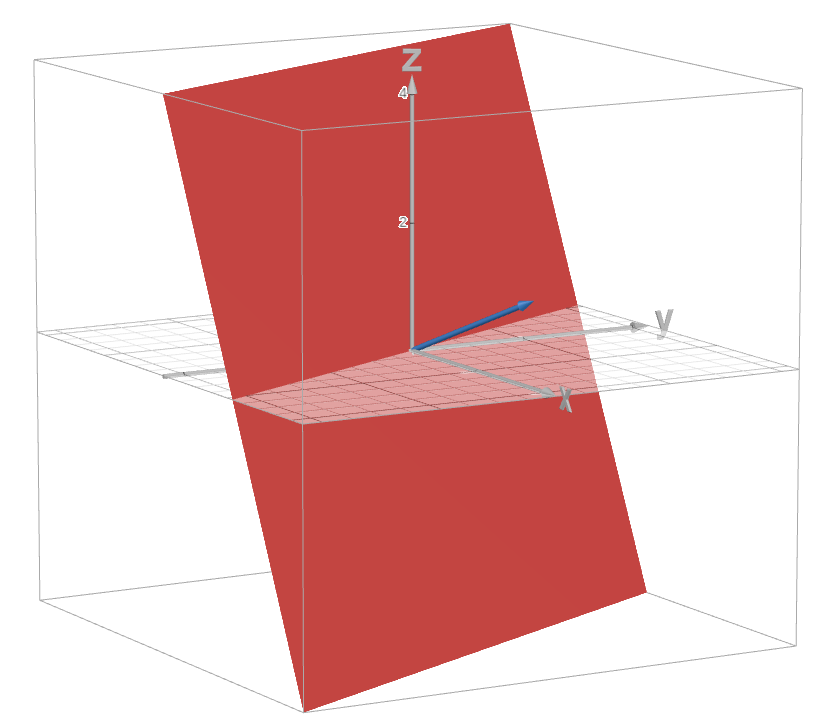
\includegraphics[scale=0.3]{Plane-5-3_nb8.png}
				\caption{The set P with $\mathbf{v} = (2, 1, 1)$. \href{https://www.desmos.com/3d/mboosgbu5z}{Desmos Link}}
			\end{figure}

			The subspace $\mathbb{R} \mathbf{v}$ is a line passing through the origin with direction vector $\mathbf{v}$.
				\begin{figure}[ht]
					\centering 
					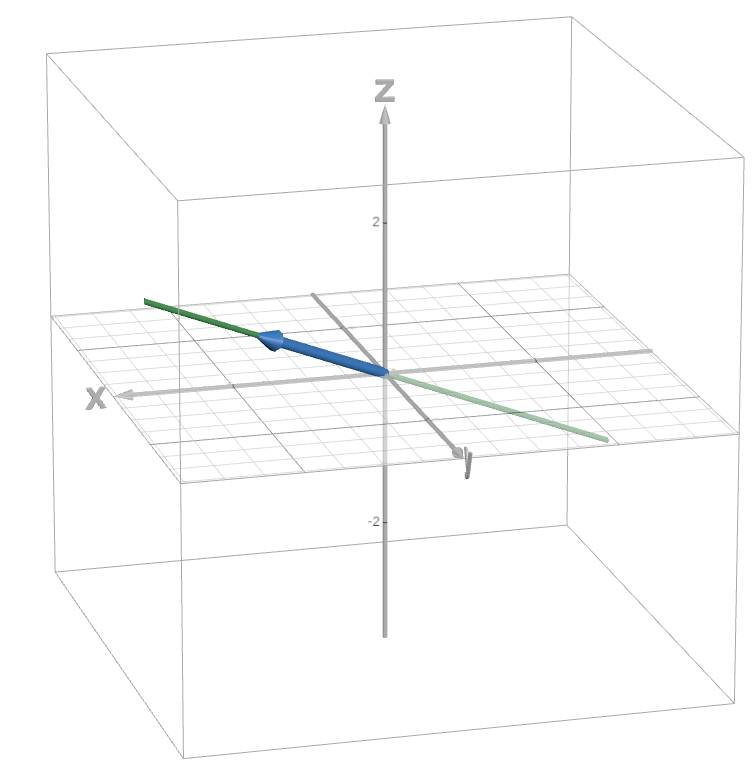
\includegraphics[scale=0.25]{line-5-3_8.png}
					\caption{The set $\mathbb{R} \mathbf{v}$ with $\mathbf{v} = (2, 1, 1)$. \href{https://www.desmos.com/3d/9zllupdlor}{Desmos Link}}
				\end{figure}

	\end{enumerate}

\spc 

\exo{8.1}{1}{10}

	\begin{enumerate}
		\item[b.] Set $\mathbf{f_1} = (2, 1)$. Then
			\[
				\mathbf{f_2} = (1, 2) - \frac{(1, 2) \cdot (2, 1)}{\Vert (2, 1) \Vert^2} (2, 1) = (-3/5, 6/5 ) .
			\]
		We then have $\{ \mathbf{f_1} , \mathbf{f_2} \}$ is a new basis of $\mathbb{R}^2$ that is orthogonal. 
		\item[c.] Set $\mathbf{f_1} = (1, -1, 1)$. Then, 
			\[
				\mathbf{f_2} = (1, 0, 1) - \frac{(1, -1, 1) \cdot (1, 0, 1)}{\Vert (1, -1, 1) \Vert^2} (1, -1, 1) = (1/3, 2/3, 1/3) 
			\]
		and
			\begin{align*}
				\mathbf{f_3} &= (1, 1, 2) - \frac{ (1, 1, 2) \cdot (1, -1, 1)}{ \Vert (1, -1, 1) \Vert^2} (1, -1, 1) - \frac{  (1, 1,2) \cdot (1/3, 2/3, 1/3)}{\Vert (1/3, 2/3, 1/3 ) \Vert^2} (1/3, 2/3, 1/3 ) \\ 
				&= (-1/2, 0, 1/2) 
			\end{align*}
		Hence $\{ (1, -1, 1), (1/3, 2/3, 1/3) , (-1/2, 0, 1/2 ) \}$ is a new basis for $\mathbb{R}^3$ that is orthogonal.
	\end{enumerate}

\spc

\exo{8.1}{4a}{10}

We notice that $(1, 1, 1)$ and $(0, 1, 1)$ are linearly independent. We can use the Gram-Schmidt Process to find an orthogonal basis for $U$. 

We set $\mathbf{f_1} = (1, 1, 1)$ and
	\[
		\mathbf{f_2} = (0, 1, 1) - \frac{(0, 1, 1) \cdot (1, 1, 1)}{3} (1, 1, 1) = (-2/3, 1/3, 1/3) .
	\]
Hence, $\{ (1, 1, 1) , (-2/3, 1/3, 1/3) \}$ is a new orthogonal basis for $U$.

\spc 

\exo{10.1}{23}{5}

We have
	\begin{align*}
		\Vert \mathbf{v} + \mathbf{w} \Vert^2 &= \left\langle \mathbf{v} + \mathbf{w} , \mathbf{v} + \mathbf{w} \right\rangle \\ 
		&= \left\langle \mathbf{v} + \mathbf{w} , \mathbf{v} \right\rangle + \left\langle \mathbf{v} + \mathbf{w} , \mathbf{w} \right\rangle \\ 
		&= \left\langle \mathbf{v} , \mathbf{v} \right\rangle + \left\langle \mathbf{w} , \mathbf{v} \right\rangle + \left\langle \mathbf{v} , \mathbf{w} \right\rangle + \left\langle \mathbf{w} , \mathbf{w} \right\rangle \\ 
		&= \Vert \mathbf{v} \Vert^2 + \left\langle \mathbf{v} , \mathbf{w} \right\rangle + \left\langle \mathbf{v} , \mathbf{w} \right\rangle + \Vert \mathbf{w} \Vert^2 \\ 
		&= \Vert \mathbf{v} \Vert^2 + 2 \left\langle \mathbf{v} , \mathbf{w} \right\rangle + \Vert \mathbf{w} \Vert^2 .
	\end{align*}
Similarly, we get
	\begin{align*}
		\Vert \mathbf{v} - \mathbf{w} \Vert^2 &= \left\langle \mathbf{v} - \mathbf{w} , \mathbf{v} - \mathbf{w} \right\rangle \\ 
		&= \left\langle \mathbf{v} - \mathbf{w} , \mathbf{v} \right\rangle + \left\langle \mathbf{v} + \mathbf{w} , -\mathbf{w} \right\rangle \\ 
		&= \left\langle \mathbf{v} , \mathbf{v} \right\rangle + \left\langle -\mathbf{w} , \mathbf{v} \right\rangle + \left\langle \mathbf{v} , -\mathbf{w} \right\rangle + \left\langle -\mathbf{w} , -\mathbf{w} \right\rangle \\ 
		&= \Vert \mathbf{v} \Vert^2 - \left\langle \mathbf{w} , \mathbf{v} \right\rangle - \left\langle \mathbf{v} , \mathbf{w} \right\rangle + \left\langle \mathbf{w} , \mathbf{w} \right\rangle \\
		&= \Vert \mathbf{v} \Vert^2 - \left\langle \mathbf{v} , \mathbf{w} \right\rangle - \left\langle \mathbf{v} , \mathbf{w} \right\rangle + \Vert \mathbf{w} \Vert^2 \\ 
		&= \Vert \mathbf{v} \Vert^2 - 2 \left\langle \mathbf{v} , \mathbf{w} \right\rangle + \Vert \mathbf{w} \Vert^2 .
	\end{align*}
Therefore,
	\[
		\frac{1}{2} \Big( \Vert \mathbf{v} + \mathbf{w} \Vert^2 + \Vert \mathbf{v} - \mathbf{w} \Vert^2 \Big) = \frac{1}{2} \Big( 2 \Vert \mathbf{v} \Vert^2 + 2\Vert \mathbf{w} \Vert^2 \Big) = \Vert \mathbf{v} \Vert^2 + \Vert \mathbf{w} \Vert^2 .
	\]

\end{document}